\documentclass{book}

\usepackage{Typocaps,lettrine}
\usepackage{graphicx}
\usepackage{subfig}
\usepackage{mathtools}
\renewcommand\LettrineFontHook{\Typocapsfamily}

\DeclarePairedDelimiter\abs{\lvert}{\rvert}%
\DeclarePairedDelimiter\norm{\lVert}{\rVert}%


\title{The little book of graph notes}

\begin{document}
\maketitle
\chapter{A starting point}
\lettrine[lines=4]{G}{raphs} do things and stuff.  They have recieved a great
deal of attention lately because they can model real world \textit{relationships}.  But what is
a graph?  

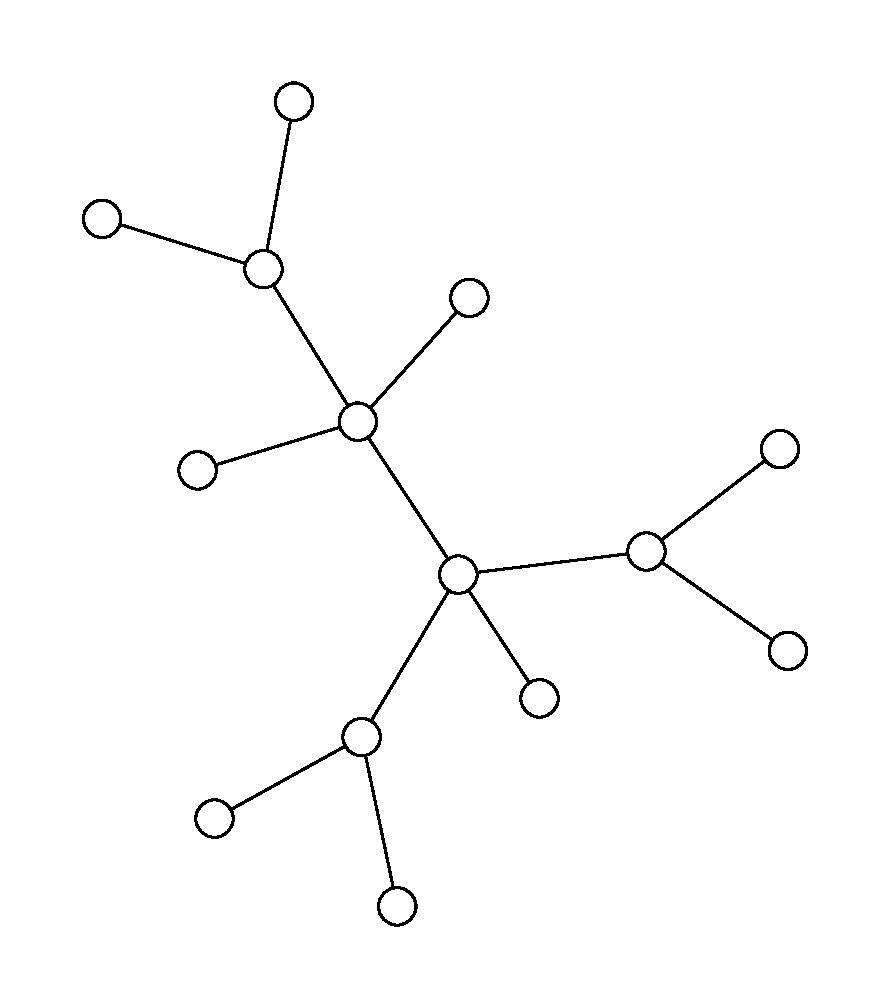
\includegraphics[width=0.4\textwidth]{tree.pdf}

\begin{figure}%
    \centering
    \subfloat[k5]{{\includegraphics[width=0.4\textwidth]{k5.pdf} }}%
    \qquad
    \subfloat[k5 again]{{\includegraphics[width=0.4\textwidth]{k5.pdf} }}%

    \subfloat[k5 again]{{\includegraphics[width=0.4\textwidth]{k5.pdf} }}%
    \caption{side by side graphs}%
    \label{fig:k5}%
\end{figure}

\chapter{Forest for the trees}
\lettrine[lines=4]{T}{rees} are just graphs. There are lots more to say about trees but that is
your job not mine. I already said some stuff once.

\end{document}
